% !TeX program = pdflatex
% !BIB program = bibtex
% Template LaTeX file for DAFx-19 papers

%------------------------------------------------------------------------------------------
%  !  !  !  !  !  !  !  !  !  !  !  ! user defined variables  !  !  !  !  !  !  !  !  !  !  !  !  !  !
% Please use these commands to define title and author(s) of the paper:
\def\papertitle{A Comparison of Virtual Analog Modelling Techniques for Desktop and Embedded Implementations}
\def\paperauthorA{Jatin Chowdhury}

% Authors' affiliations have to be set below

%------------------------------------------------------------------------------------------
\documentclass[twoside,a4paper]{article}
\usepackage{dafx_19}
\usepackage{amsmath,amssymb,amsfonts,amsthm}
\usepackage{euscript}
\usepackage[latin1]{inputenc}
\usepackage[T1]{fontenc}
\usepackage{ifpdf}

\usepackage[english]{babel}
\usepackage{caption}
\usepackage{subfig} % or can use subcaption package
\usepackage{xcolor}

\setcounter{page}{1}
\ninept

\usepackage{times}
% Saves a lot of ouptut space in PDF... after conversion with the distiller
% Delete if you cannot get PS fonts working on your system.

% pdf-tex settings: detect automatically if run by latex or pdflatex
\newif\ifpdf
\ifx\pdfoutput\relax
\else
   \ifcase\pdfoutput
      \pdffalse
   \else
      \pdftrue
\fi

\ifpdf % compiling with pdflatex
  \usepackage[pdftex,
    pdftitle={\papertitle},
    pdfauthor={\paperauthorA},
    colorlinks=false, % links are activated as colror boxes instead of color text
    bookmarksnumbered, % use section numbers with bookmarks
    pdfstartview=XYZ % start with zoom=100% instead of full screen; especially useful if working with a big screen :-)
  ]{hyperref}
  \pdfcompresslevel=9
  \usepackage[pdftex]{graphicx}
  \usepackage[figure,table]{hypcap}
\else % compiling with latex
  \usepackage[dvips]{epsfig,graphicx}
  \usepackage[dvips,
    colorlinks=false, % no color links
    bookmarksnumbered, % use section numbers with bookmarks
    pdfstartview=XYZ % start with zoom=100% instead of full screen
  ]{hyperref}
  % hyperrefs are active in the pdf file after conversion
  \usepackage[figure,table]{hypcap}
\fi

% My packages
\usepackage{tikz}
\usepackage[american]{circuitikz}
% \usetikzlibrary{dsp,chains}
\usepackage{tkz-euclide}
\usepackage{cleveref}
\usepackage{siunitx}

\usepackage{listings}
\definecolor{codegreen}{rgb}{0,0.6,0}
\definecolor{codegray}{rgb}{0.5,0.5,0.5}
\definecolor{codepurple}{rgb}{0.58,0,0.82}
\definecolor{backcolour}{rgb}{0.95,0.95,0.92}
 
\lstdefinestyle{mystyle}{
    backgroundcolor=\color{backcolour},   
    commentstyle=\color{codegreen},
    keywordstyle=\color{magenta},
    numberstyle=\tiny\color{codegray},
    stringstyle=\color{codepurple},
    basicstyle=\footnotesize,
    columns=flexible,
    breakatwhitespace=false,         
    breaklines=true,                 
    captionpos=b,                    
    keepspaces=true,                               
    showspaces=false,                
    showstringspaces=false,
    showtabs=false,                  
    tabsize=4
}
 
\lstset{style=mystyle}

\DeclareMathAlphabet{\mathpzc}{OT1}{pzc}{m}{it}
\newcommand{\z}{\mathpzc{z}}

\title{\papertitle}

\affiliation{
\paperauthorA \,}
{\href{http://ccrma.stanford.edu}{Center for Computer Research in Music and Acoustics} \\ Stanford University \\ Palo Alto, CA \\ {\tt \href{mailto:jatin@ccrma.stanford.edu}{jatin@ccrma.stanford.edu}}}

\begin{document}
% more pdf-tex settings:
\ifpdf % used graphic file format for pdflatex
  \DeclareGraphicsExtensions{.png,.jpg,.pdf}
\else  % used graphic file format for latex
  \DeclareGraphicsExtensions{.eps}
\fi

\graphicspath{{./Figures/}}

\maketitle
%
\begin{abstract}
In this writing, we develop a virtual analog model of the Klon Centaur
guitar pedal circuit, comparing various circuit modelling techniques.
The techniques analyzed include traditional modelling techniques such
as nodal analysis and Wave Digital Filters, as well a machine-learning
technique using recurrent neural networks. We examine these techniques
in the contexts of two use cases: an audio ``plug-in'' designed to be
run on a consumer-grade desktop computer, and a guitar pedal-style effect
running on an embedded device. Finally, we discuss the advantages and
disdvantages of each technique for modelling different circuits, and
targetting different platforms.
\end{abstract}

\section{Introduction}
The Klon Centaur is an overdrive guitar pedal designed by Bill
Finnegan in the early 1990's, that has developed cult acclaim
amongst guitarists \cite{Finnegan}. The circuit is notable for
producing ``transparent distortion'' \cite{electrosmash},
a term used to describe the way the pedal seems to add distortion
to a guitar's sound without otherwise affecting the tone. While
the original manufacturing run of the pedal ended in 2004, many
``clones'' of the pedal have been produced by other manufacturers,
adding to its cult following.
\newline\newline
Circuit modelling is typically broken down into ``white-box'' and
``black-box'' approaches \cite{Germain}. A ``white-box'' approach
uses knowledge of the internal mechanisms of the circuit, often
modelling the physical interactions of the electrical components.
Popular white-box methods include nodal analysis \cite{Yeh},
Port-Hamiltonian analysis \cite{PortHamiltonian}, Wave Digital
Filters \cite{Fettweis,KurtThesis}, and nonlinear state space
analysis \cite{StateSpace}.
\newline\newline
``Black-box'' circuit modelling methods generally use measurements
taken from the circuit being modelled and attempt to model the
response of the circuit without knowledge of the internal workings
of the system. Traditional black-box techniques include impulse
response measurements \cite{sasp} and extensions thereof, including
the Weiner-Hammerstein method \cite{Germain}. Recently, researchers
have begun using machine learning methods for black-box modelling.
In \cite{WaveNetVA}, the authors use a WaveNet style architecture
to generate an output signal sample-by-sample. In \cite{NLML} the
authors use a deep fully-connected networks to approximate nonlinear
state-space solutions for a circuit, effectively a ``grey-box'' approach.
Finally, in \cite{VArnn} the authors use a recurrent neural network
to model the behavior of audio circuits with control parameters.


\section{Traditional Circuit Modelling Techniques}
First, we examine the use of traditional circuit modelling techniques,
specifically nodal analysis and Wave Digital filters, using
sub-circuits from the Klon Centaur as examples.

\subsection{Nodal Analysis}
The process for creating a digital model of a circuit using nodal
analysis is as follows:
\begin{enumerate}
    \item Convert the circuit into the Laplace domain.
    \item Form a Laplace domain transfer function of the circuit.
    \item Use a conformal map to transform the circuit into the digital domain.
\end{enumerate}
%
As an example circuit, we examine the Tone Control circuit from the
Klon Centaur (see \cref{fig:ToneControl}).
%
\begin{figure}
    \centering
    \begin{circuitikz} \draw
        (0, 0) node[op amp] (opamp) {}
        (opamp.+) to[short, l_=+4.5V,-o] (-1.2, -1.0)
        (opamp.-) to[R, l=R22] (-3, 0.5)
        to[short, l=Vin,-o] (-3.5, 0.5)
        (-3, 0.5) to[R, l=R21] (-3, 2.0)
        (-3, 4.0) to[american potentiometer, l_=RV2, n=mypot] (-3, 2.0)
        (mypot.wiper) to[C, l=C14] (-1.2, 3.0)
        (opamp.-) -- (-1.2, 3.0)
        to[R, l=R24] (1.5, 3.0)
        (-3, 4.0) to[R, l=R23] (1.5, 4.0)
        -- (1.5, 0.0)
        (opamp.out) -- (1.5, 0.0) to[short, l_=Vout,-o] (2.5, 0.0)
      ;
    \end{circuitikz}
    \caption{\label{fig:ToneControl}{\it Klon Centaur Tone Control Circuit}}
\end{figure}
%
The first step is to convert the circuit into the Laplace domain, using
the Laplace variable $s = j\omega$. The impedances for each principle
circuit component: resistors ($Z_R$), capacitors ($Z_C$), and inductors
($Z_L$), are as follows:
\begin{equation}
    Z_R = R, \quad Z_C = \frac{1}{Cs}, \quad Z_L = Ls
\end{equation}
%
From there, using linear circuit theory, one can construct a Laplace
Domain transfer function for the circuit. Note that this assumes an
ideal operational amplifier operating in its linear region. For more
information on this process, see \cite{Maby}. For the tone control
circuit, the Laplace domain transfer function can be written as:
\begin{equation}
    \frac{V_{out}(s)}{V_{in}(s)} = {\scriptscriptstyle \frac{C_{14}\left(\frac{1}{R_{22}} + \frac{1}{R_{21} + R_{v2b}}\right)s
    + \frac{1}{R_{22}}\left(\frac{1}{R_{21} + R_{v2b}} + \frac{1}{R_{23} + R_{v2a}}\right)}{
      C_{14}\left(\frac{1}{R_{23} + R_{v2a}} + \frac{1}{R_{24}}\right)s
    + \frac{-1}{R_{24}}\left(\frac{1}{R_{21} + R_{v2b}} + \frac{1}{R_{23} + R_{v2a}}\right)}}
\end{equation}
%
Note that we refer to the the section of potentiometer $R_{v2}$ that is
above the wiper as $R_{v2a}$, and the section below as $R_{v2b}$, and that
we ignore the DC offset created by the $4.5$V voltage source at the positive
terminal of the op-amp.
\newline\newline
Next we use a conformal map to transform the transfer function from the
Laplace domain to the z-plane where it can be implemented as a digital
filter. The most commonly used conformal map is the bilinear transform,
defined as
\begin{equation}
    s \leftarrow \frac{2}{T} \frac{1 - z^{-1}}{1 + z^{-1}}
\end{equation}
%
Where $T$ is the sample period of the digital system. For more
information on the use of the bilinear transform to digitize an
analog system, see \cite{pasp}. The resulting filter is known as a
``high-shelf'' filter, that accentuates high frequency content in
the signal. The resulting frequency response of the digital model,
validated against the response of the analog circuit is shown in
\cref{fig:ToneFreq}.
\begin{figure}
    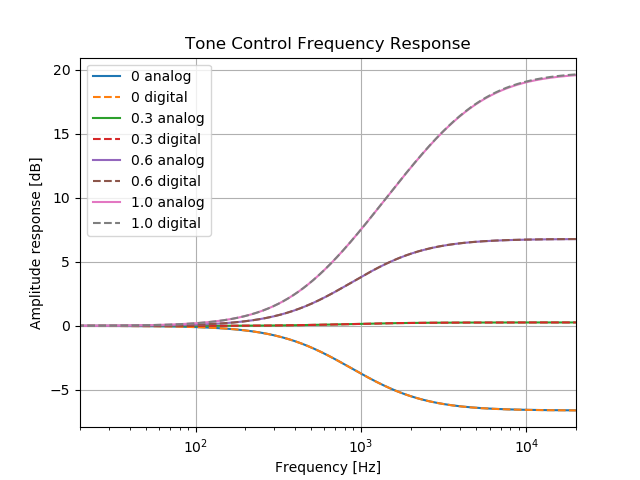
\includegraphics[width=0.5\textwidth]{ToneFreq.png}
    \caption{\label{fig:ToneFreq} {\it Tone control frequency response
    at various values of the Treble parameter, comparing the responses
    of the analog filter with the digital model.}}
\end{figure}

\subsubsection{Advantages and Limitations}
The advantages of nodal analysis are that the circuit model
is simple and computationally efficient. The model can be constructed
with minimal knowledge of simple circuit theory, and basic understanding
of digitial signal processing. The main disdvantage is that nodal analysis
cannot be used for nonlinear circuits, though it can be extended
to model this class of circuits through modified nodal analysis (MNA)
\cite{MNA}. Another disadvantage of nodal analysis-based methods
is that (typically) large portions of the system need to be recomputed
when a circuit element is changed, such as a potentiometer. While this
computation is fairly simple in the example shown here, it can become
vastly more difficult for more complex systems.

\subsection{Wave Digital Filters}
The Wave Digital Filter (WDF) formalism allows circuits to be modelled in
modular and flexible manner. Originally developed by Alfred Fettweis
in the 1970's \cite{Fettweis}, WDFs have recently gained popularity in
modelling audio circuits, and have been extended to model a wider class
of circuits \cite{KurtThesis}. The WDF formalism defines each circuit element
as a port with some characteristic resistance $R_0$, and uses wave variables
passing through each port, rather than the typical voltage and current variables.
The incident wave at a certain port is defined as:
\begin{equation}
    a = v + R_0 i
\end{equation}
where $v$ is the voltage across the port, and $i$ is the current passing
through the port. The reflected wave is similarly defined as:
\begin{equation}
    b = v - R_0 i
\end{equation}
A Wave Digital Filter defines circuit elements (resistors, capacitors,
inductors, etc.) in the wave domain, and allows the elements to be connected
by series and parallel adaptors also defined in the wave domain. The
full derivation of these WDF elements is given in \cite{Fettweis} and
\cite{KurtThesis}. 
\newline\newline
Once each circuit element and adaptor has been defined, they are connected
together in a strcuture often referred to as a WDF tree. As an example,
we examine the ``feed-forward network 1'' from the Klon Centaur circuit
(see \cref{fig:ff1}).

\begin{figure}
    \centering
    \begin{circuitikz} \draw
        (0, 0) node[short, l=Vin] {}
        to[C, l=C3, o-] (2, 0)
        to[R, l=R7]     (3.25, 0)
        to[R, l=R19]    (6, 0)
        to[V, l=4.5V]   (6, -1.5)
        (3.5, 0) to[C, l=C16] (3.5, -1.5)
        (3.5, -1.25) node[ground]() {}
        (6.0, -1.25) node[ground]() {}
      ;
    \end{circuitikz}
    \caption{\label{fig:ff1}{\it Klon Centaur Feed-Forward Network 1 Circuit}}
\end{figure}
%
The corresponding WDF tree is given below. @TODO\dots
Also shwo simulation results. @TODO\dots
\newline\newline
\begin{figure}
    \centering
    \caption{\label{fig:wdftree}{\it WDF tree for the Klon Centaur Feed-Forward Network 1 Circuit.}}
\end{figure}
%
\subsubsection{Advantages and Limitations}
The primary advantage of the Wave Digital approach is its modularity.
The ability to construct a circuit model with each circuit component
treated completely independently in the digital domain opens up many
interesting possibilities for circuit prototyping, modelling circuit-bent
instruments and more. Additionally, this modularity allows each circuit
component to be discretized separately, even using different conformal
maps, which can improve model behavior for certain classes of circuits
(see \cite{Germain}). Finally, the separability of components means than
when a component is changed (e.g. a potentiometer), the component change
is propagated so that only components with behavior that depends on the
impedance of the changed component need to be recomputed.
\newline\newline
The main disdvantage of WDFs is its difficulty in handling circuits with
complex topologies, or multiple nonlinearities. While the recent addition
of $\mathcal{R}$-type adaptors to the Wave Digital formalism \cite{KurtThesis}
has begun to make these circuits tractable, the WDF models of these types of
circuits are significantly more computationally complex, and somewhat
compromise the modularity of the system.

\section{Recurrent Neural Network Model}
While several styles of machine-learning based models are available for
modelling analog audio circuitry \cite{WaveNetVA,NLML,MartinezReissDNN},
we choose the recurrent neural network approach developed in \cite{VArnn}
as our starting point. Using a recurrent neural network (RNN) allows the for a
significantly smaller neural network than would be possible with a traditional
deep neural network or convolutional neural network, meaning that the network
can be evaluated much faster for real-time use, while maintaining a smaller
memory footprint (an important advantage on embedded platforms). Additionally,
recurrent neural networks are a sensible candidate for modelling distortion
circuits, particularly circuits with stateful behavior, given the fact that
recurrent network building blocks, such as gated recurrent units, themselves
resemble audio distortion effects, and can directly be used as such
\cite{chowdhury:complexNL:2020}. Finally, the model proposed in \cite{VArnn}
allows for the inclusion of control parameters into the model, such as
potentiometer positions, helping to solve a persistent limitation of
black-box style circuit models.
\newline\newline
In the following paragraphs, we outline the use of an RNN for modelling
the gain stage circuit from the Klon Centaur pedal. While our model
is similar to the model used in \cite{VArnn}, it differs in some
notable ways. For instance, the model described in \cite{VArnn} accepts
the values of control parameters to the circuit as inputs to the RNN,
however we were unable to successfully train a network in this fashion.
Instead, we construct separate networks for five different values of the
``Gain'' parameter, and fade between the outputs of the networks in
real-time in the final implementation of the model. Other differences are
outlined further below.

\subsection{Model Architecture}
The model architecture described in \cite{VArnn} consists of a single recurrent
layer followed by a fully connected layer consisting of a single ``neuron''
(see \cref{fig:rnn_arch}). In our models, we use a recurrent layer made up
of 8 Gated Recurrent Units. For training, all models are implemented in
\texttt{Python} using the \texttt{Keras} framework \cite{chollet2015keras}.
%
\begin{figure}
    \centering
    \begin{tikzpicture}[node distance=1.5cm]
        \tikzset{
            mynode/.style = {rectangle, rounded corners, line width=0.8pt, minimum width=2cm, minimum height=0.75cm, text centered, draw=black, fill=white},
            arrow/.style = {thick,->,>=stealth}
        }
        \node (input) {Input $x[n]$};
        \node (rlayer) [mynode, right of=input, xshift=1.25cm] {Recurrent Layer};
        \coordinate[right of=rlayer, xshift=0.5cm] (h0) ;
        \node (h0Label) [right of=h0, xshift=-0.15cm] {Current State $h[n]$};
        \node (z1) [rectangle, draw=black, below of=h0, yshift=0.5cm] {$z^{-1}$};
        \coordinate[below of=rlayer, yshift=0.5cm] (h1);
        \node (h1Label) [below of=h1, yshift=1.15cm] {Previous State $h[n-1]$};

        \draw [arrow] (input) -- (rlayer);
        \draw [thick] (rlayer) -- (h0);
        \draw [arrow] (h0) -- (z1);
        \draw [thick] (z1) -- (h1);
        \draw [arrow] (h1) -- (rlayer);

        \node (dense) [mynode, above of=rlayer] {Fully Connected Layer};
        \node (out) [above of=dense] {Output $y[n]$};
        \draw [arrow] (rlayer) -- (dense);
        \draw [arrow] (dense) -- (out);

    \end{tikzpicture}
    \caption{\label{fig:rnn_arch}{\it RNN Architecture.}}
\end{figure}
%
\subsubsection{Recurrent Layer}
Recurrent layers are typically comprised of one of two types of
recurrent units: Long Short-Term Memory units (LSTMs) or Gated
Recurrent Units (GRUs). For this application, we choose to use
GRUs \cite{gru_original} since they require fewer operations,
allowing for faster computation, and since they requre fewer weights,
thereby allowing the model to have a smaller memory footprint. The
GRU consists of three ``gates'': the update gate $z[n]$, reset gate
$r[n]$, and the new gate $c[n]$. These gates are used to compute the
cell's current output $h[n]$ from its current input $x[n]$ and previous
output $h[n-1]$ as follows:
\begin{equation}
    z[n] = \sigma(W_z x[n] + U_z h[n-1] + b_z)
\end{equation}
\begin{equation}
    r[n] = \sigma(W_r x[n] + U_r h[n-1] + b_r)
\end{equation}
\begin{equation}
    c[n] = \tanh(W_c x[n] + r[n] \circ U_c h[n-1] + b_c)
\end{equation}
\begin{equation}
    h[n] = z[n] \circ h[n-1] + (1 - z[n]) \circ c[n]
\end{equation}
%
Where $W_z,W_r,W_c$ are the kernel weights for each gate,
$U_z,U_r,U_c$ are the recurrent weights for each gate, and
$b_z,b_r,b_c$ are the biases for each gate. Note that as the
inputs and outputs to the GRU layer may be vectors, all products
in the above equations are assumed to be standard matrix-vector
products, except those Hadamard products denoted $\circ$.
%
\subsubsection{Fully Connected Layer}
A fully connected layer computes an output vector $y[n]$ from
input vector $x[n]$ as follows:
\begin{equation}
    y[n] = \alpha(W x[n] + b)
\end{equation}
%
Where $W$ is the kernel weights, $b$ is the layer bias, and $\alpha(x)$
is the layer activation. In our model, we use no activation, i.e.,
$\alpha(x) = x$.

\subsection{Training Data}
Our dataset consists of ~4 minutes of electric guitar recordings,
from a variety of electric guitars including a Fender Stratocaster
and a Gibson Les Paul. The guitars are recorded ``direct'' meaning
that the recorded signal is equivalent to the signal received by the
pedal coming directly from the guitar. Recordings were made using a
Focusrite Scarlett audio interface at 44.1 kHz. Note that this
sample rate is very low compared to that used for other neural network
models of nonlinear audio effects \cite{WaveNetVA,VArnn}, however,
this sample rate was chosen because the embedded hardware on which
the final model was implemented processes audio at this sample rate.
The recordings were then separated into segments of 0.5 seconds each,
resulting in a total of 425 segments.
\newline\newline
Since the original Klon Centaur is quite expensive, we used a SPICE
simulation of the Centaur circuit in order to obtain a ``ground truth''
reference dataset. The reference dataset measures the output voltage
of the summing amplifier from the circuit at five different values
for the ``Gain'' potentiometer.

\subsection{Training}
We trained our models on 400 of the 425 audio samples, saving 25
samples for validation. Training was performed using the Adam
optimizer \cite{Kingma2015AdamAM}, with an initial learning rate
of \num{2e-3}.

\section{Implementation}
In order to compare the virtual analog methods described above,
we construct two emulations of the Klon Centaur circuit: one emulation
using traditional circuit modelling methods, and a second using a
recurrent neural network. The Centaur circuit can be broken down
into four separable parts:
\begin{enumerate}
    \item Input Buffer
    \item Gain Stage
    \item Tone Control
    \item Output Buffer
\end{enumerate}
%
Due to their simplicity and linearity, in both emulations the input
buffer, output buffer, and tone control circuits were modelled using
nodal analysis. The ``Gain Stage'' circuit can be further broken down
into six (mostly) separable parts:
\begin{enumerate}
    \item Feed-Forward Network 1 (FF-1)
    \item Feed-Forward Network 2 (FF-2)
    \item Pre-Amp Stage
    \item Amplifier Stage
    \item Clipping Stage
    \item Summing Amplifier
\end{enumerate}
%
@TODO, circuit schematic of gain stage with parts highlighted
%
In the RNN circuit model, we treat the Gain Stage as a black box
with a single user-facing control (the ``Gain'' control). The RNN
is designed to completely replace the Gain Stage in the circuit
model. In the traditional circuit model, we use nodal analysis to
model the amplifier stage, and summing amplifier circuits.
For FF-2 and the clipping stage, we use a wave digital filter.
Since FF-1 and the pre-amp circuit share a capacitor, we construct
a joint WDF model of these two circuits, using the voltage output
from the pre-amp circuit as the input to the amplifier stage, and
the current output from FF-1 (summed with the current outputs of
FF-2 and the clipping stage) as the input to the summing amplifier.

\subsection{Audio Plugin}
Digital audio effects are often implemented as audio plugins that
can be used by mixing engineers, producers, and musicians in a
consumer digital audio workstation (DAW) software. Common plugin
formats include the Avid Audio Extension (AAX), Steinberg's Virtual
Studio Technology (VST), and Apple's Audio Unit (AU) for desktop use,
as well as Apple's Audio Unit v3 (AUv3) for mobile use. The JUCE C++
framework\footnote{\url{https://github.com/juce-framework/JUCE}} is
commonly used to create cross-platform, cross-format plugins.
\newline\newline
As a demonstration of the two circuit emulations, we construct an audio
plugin containing both models, allowing the user to switch
between the two models for comparison. The plugin is implemented using
JUCE/C++, along with a real-time Wave Digital Filter
library\footnote{\url{https://github.com/jatinchowdhury18/WaveDigitalFilters}}
for the WDF models. While the current model uses custom implementations
of the GRU and fully connected layers needed for the RNN model, in the
future, we plan to upgrade this model to use the implementations provided
by the Tensorflow Lite library\footnote{\url{https://www.tensorflow.org/lite/}}.
%
\begin{figure}
    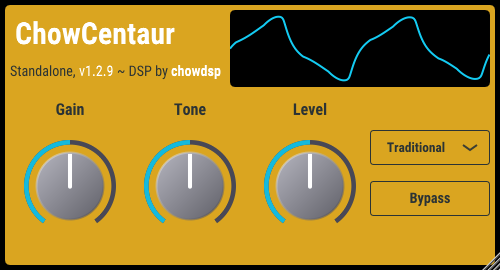
\includegraphics[width=0.5\textwidth]{Plugin.png}
    \caption{\label{fig:Plugin} {\it Audio plugin implementation
    of the Klon Centaur circuit model. Note controls for ``Gain'',
    ``Treble'', and ``Level'' analogous to the original circuit,
    as well as the ``neural'' parameter to control whether the
    emulation uses the traiditional circuit model, or the RNN model.}}
\end{figure}

\subsection{Embedded Implementation}
Digital audio effects are sometimes implemented on embedded devices
for use in stage performances, often in the form of a guitar pedal,
or synthesizer module. Deploying an audio effect on an embedded device
can be difficult, due to the constraints in processing power and memory
availability. Further, in order to achieve a more expressive performance,
musicians often prefer effects that add minimal latency to the signal,
meaning that the embedded implementation must be able to run with a
very small buffer size.
\newline\newline
We chose the Teensy 4.0 microcontroller as our embedded platform, since
it contains a reasonbly powerful floating point processor, at a relatively
low price point. The Teensy can be purchased along with an Audio Shield,
which provides 16-bit stereo audio input/output at 44.1 kHz sampling rate.
The Teensy has gained popularity in the audio community due to
the Teensy Audio Library\footnote{\url{https://www.pjrc.com/teensy/td_libs_Audio.html}}
that contains useful audio DSP functionality, as well as the Faust
programming language which allows audio effects and synthesizers made in
Faust to be exported for use on the Teensy \cite{Michon2019RealTA}.


\section{Results}
asdjfahlsk


\section{Conclusion}
In this writing\dots



\section{Acknowledgments}
%
The author would like to thank Pete Warden and the EE292 class at
Stanford University for inspiring this project, as well as Julius
Smith, Kurt Werner, and Jingjie Zhang for assistance with Wave
Digital Filter modelling.

%\newpage
\nocite{*}
\bibliographystyle{IEEEbib}
\bibliography{references}

\end{document}
